\subsubsection{Erster Test des Gehäuses}\label{hw_case_ersterTest}
Zur Erstellung des Gehäuses haben wir die Maße des Bildschirms als Anhaltspunkt genommen. 
Die erste Messung haben wir mit einem Meterstab durchgeführt.
Der Bildschirm hatte an der Hinterseite eine Erhebung, weshalb wir diese ebenfalls ausgemessen haben. 
Die Maße beliefen sich nach der ersten Messung auf:
\begin{itemize}
	\item 255,5 mm Breite
	\item 167 mm Höhe
	\item Kantenradius 10 mm
\end{itemize}
\begin{figure}[H]
	\includegraphics[width=1\textwidth]{img/abmessungen_gehäuse.jpg}
	\caption[Abmessungen Bildschirm Rückseite]{Abmessungen Bildschirm Rückseite}
	\label{fig:screen-back-01}
\end{figure}
\noindent Anhand dieser Maße haben wir dann in Fusion 360 eine Grundplanzeichnung erstellt und ein 3D-Modell gefertigt.\par	
\noindent Nach Überprüfung der Maße haben wir dann allerdings festgestellt, dass der zur Verfügung stehende 3D-Drucker, ein Ender 3 Pro der Firma Creality3D, ein maximales Druckvolumen von 235x235x220mm besitzt und somit das Gehäuse nicht wie ursrpünglich geplant aus einem Stück sondern in mehreren Teilen gedruckt werden muss. 
Hierfür haben wir eine Änderung der Konstruktion durchgeführt. 
Das Gehäuse besteht nun aus vier Teilen, zwei davon bilden jeweils die Seitenwände während zwei den Deckel des Gehäuses bilden. 
Die Teile werden mit langen M3 Senkkopfschrauben verbunden, die zusätzlich als Verschluss des Gehäuses dient.\par
\begin{figure}[H]
	\includegraphics[width=1\textwidth]{img/druck_gehäuse_001.png}
	\caption[Platzierung der beiden Gehäusewände in CURA]{Platzierung der beiden Gehäusewände in CURA}
	\label{fig:print-case-test_01}
\end{figure}
\begin{figure}[H]
	\includegraphics[width=1\textwidth]{img/druck_gehäuse_002.png}
	\caption[Verschiebung der Modelle entlang der Z-Achse um 45mm]{Verschiebung der Modelle entlang der Z-Achse um 45mm}
	\label{fig:print-case-test_02}
\end{figure}
\begin{figure}[H]
	\includegraphics[width=1\textwidth]{img/druck_gehäuse_002.png}
	\caption[Slicen der Modelle]{Slicen der Modelle}
	\label{fig:print-case-test_03}
\end{figure}
\begin{figure}[H]
	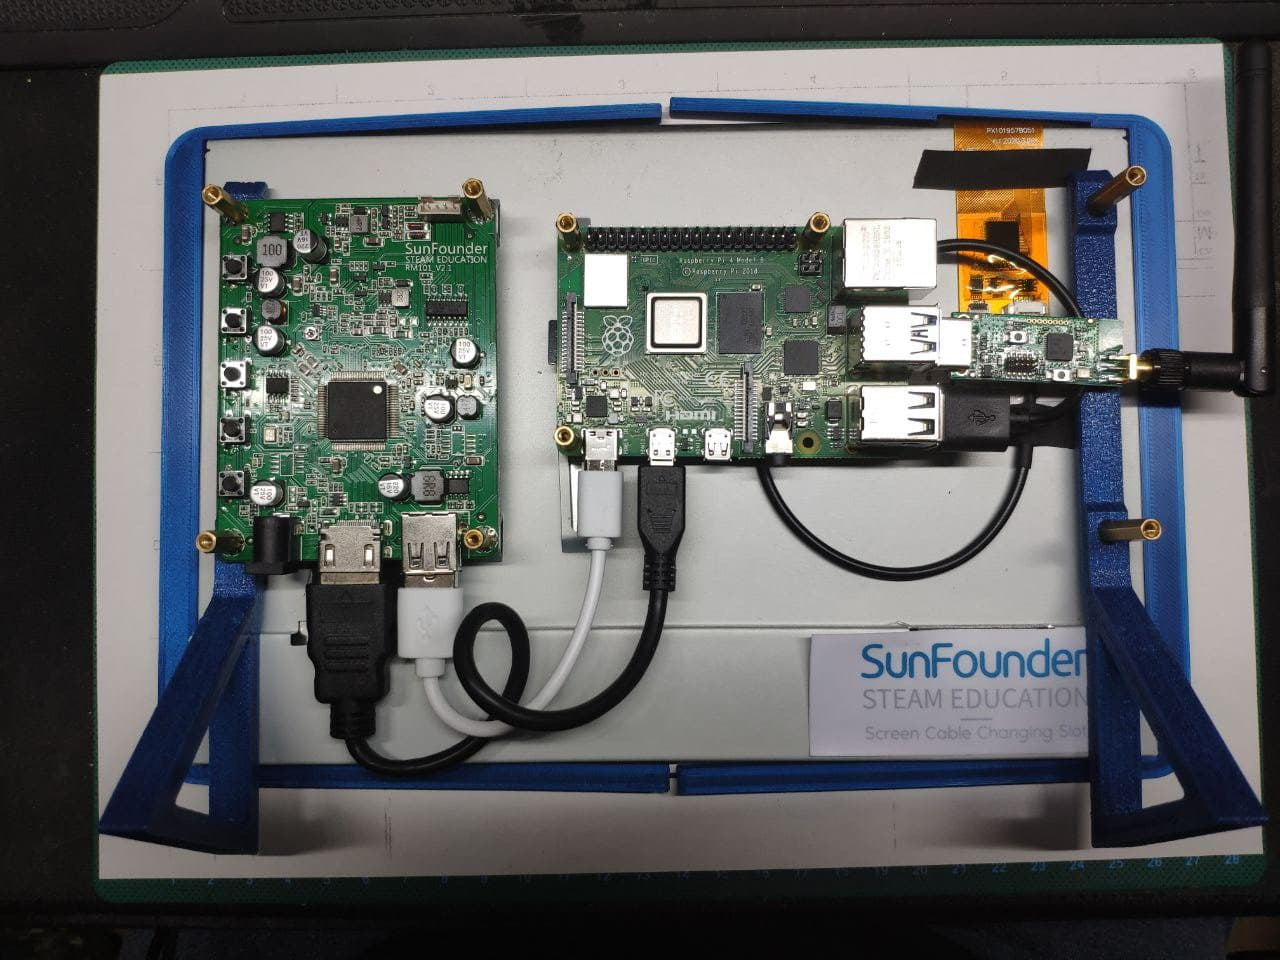
\includegraphics[width=1\textwidth]{img/testdruck_an_bildschirm.jpg}
	\caption[Passung des Testdrucks]{Passung des Testdrucks}
	\label{fig:print-case-test_04}
\end{figure}
\noindent Um die Genauigkeit der Konstruktion zu testen, haben wir eine 5 Millimeter hohe Schablone zum Testen ausgedruckt, die an den Bildschirm angelegt werden kann. 
Diese entstand mit Hilfe des Slicers CURA (vgl. Abb. \ref{fig:print-case-test_01}: \nameref{fig:print-case-test_01}), in dem die Modelle der beiden Seitenteile so angeordnet wurden, dass lediglich 5 Millimeter des Teils im druckbaren Bereich des Druckers verblieben (vgl. Abb. \ref{fig:print-case-test_02}: \nameref{fig:print-case-test_02}). Anschließend haben wir die Teile noch auf dem Druckbett zentriert (vgl. Abb. \ref{fig:print-case-test_03}: \nameref{fig:print-case-test_03}).\\
\noindent Nach dem Ausdrucken war klar, dass die Maße des ersten Versuchs nicht genau genug waren (vgl. Abb. \ref{fig:print-case-test_04}: \nameref{fig:print-case-test_04}, weshalb wir zum Ausmessen ,,genauere'' Messwerkzeuge zur Hand nahmen \footnote{Digitaler Messschieber mit einer Nachkommastelle \& einer  Genauigkeit von $\pm$ 0.2mm}